\section{Coherent states of the harmonic oscillator}
We know that quantum mechanics must yield the same results as classical mechanics in the limiting casr where the harmonic 
oscillator has an energy much greater than the quantum $\hbar\omega$.

It is possible to construct quantum mechanics states leading to physical predictions which are almost identical to the classical ones, at least 
for a macroscopic oscillator? Such quantum sistems do exist: they are coherent linear superpositions of all the states $\ket{\varphi_n}$. We shall 
call them \bfemph{quasi-classical states} or coherent states of the harmonic oscillator.

It is important to understand, in the framework of quantum mechanics, how to move gradually from the case in which thee results given by the classical approximation 
are sufficient to the case in which quantum effects are preponderant.

The position, momentum, and energy of a harmonic oscillator are described in QM by operators which do not commute.
It is not possible to construct a state in which they are all perfectly well-defined.

Theregore, we shall only look for a state vector such that for all $t$, the mean values $\braket{X}$, $\braket{P}$, and $\braket{H}$ are 
as close as possible to the corresponding classical values: the compromise if then that none of these three observables is perfectly known.
Nevertheless, the rms deviation $\Delta X$, $\Delta Y$, and $\Delta H$ are, in the macroscopic limit, completely negligible.
%%
\subsection{Quasi-classical states}
%
\subsubsection{Introducing $\alpha_0$ to characterize a classical motion}
The classical quantitites of motion of a 1D harmonics oscillator of mass $m$ and angular frrequency $\omega$ are 
\begin{align}
    \text{Equations of motion for CHO}\qquad\highlight{\begin{array}{l}
        \dfrac{d}{dt}x(t)=\dfrac{1}{m}p(t)\\
        \dfrac{d}{dt}p(t)=-m\omega^2x(t)
    \end{array}}.
\end{align}
The classical state of the HO is determined at time $t$ when we know its position $x(t)$ and its momentum $p(t)$.
We shall therefore combine them into a single complex number $\alpha(t)$ given by:
\begin{align}
    \text{Displacement coordinate}\qquad\highlight{\alpha(t)=\frac{1}{\sqrt{2}}\left(\frac{x(t)}{\sigma}+i\frac{\sigma p(t)}{\hbar}\right)\quad(-)}.
\end{align}
Then, the equations of motions turn to 
\begin{align}
    \frac{d}{dt}\alpha(t)=-i\omega\alpha(t)\longrightarrow\highlight{\alpha(t)=\alpha_0e^{-i\omega t},\quad \alpha_0=\alpha(0)}
    \label{eq:timeevolaclassic}
\end{align}
We can plot this evolution in a geometrical representation of the evolution of the state of the system through the \bfemph{phase-space diagram} 
as shown in the following figure.
\begin{figure}[h!]
    \centering
    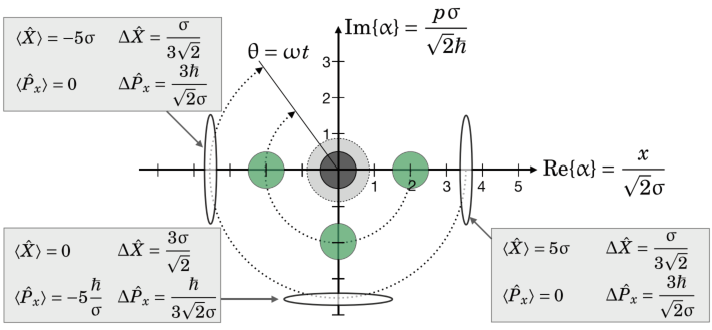
\includegraphics[width=.7\columnwidth]{PartOne/ChapterThree/phasespacediagram.png}
    \caption{Illustration of four HO states in the phase-space diagram: black=ground state, gray=first excited state, 
    ovals=squeezed state, green=coherent state.}
\end{figure}
According to the solution of the ODE, we have 
\begin{align}
    x(t)=\frac{1}{\sqrt{2}}(\alpha_0e^{-i\omega t}+\alpha_0^*e^{i\omega t}),\quad p(t)=-\frac{i}{\sqrt{2}}(\alpha_0e^{-i\omega t}-\alpha_0^*e^{i\omega t}).
\end{align}
As for the classcal energy $\mathcal{H}$ of the system, it is constant in time and equal to:
\begin{align*}
    \mathcal{H}=\frac{1}{2m}p(0)^2+\frac{1}{2}m\omega^2x^2(0)=\frac{\hbar\omega}{2}\left[\left(\frac{x(0)}{\sigma}\right)^2+\left(\frac{\sigma p(0)}{\hbar}\right)^2\right]=\hbar\omega|\alpha_0|^2.
\end{align*}
For a macroscopic oscillator, the energy $\mathcal{H}$ is much greater than the quantum $\hbar\omega$, so 
\begin{align}
    \text{Macroscopic regime}\qquad\highlight{|\alpha_0|\gg1}.
\end{align}


%
\subsubsection{Conditions defining quasi-classical states}
We are looking for a quantum mechanical state for which at every instant the mean values $\braket{X}$, $\braket{P}$, and $\braket{H}$ are practically equal to the values of 
$x$, $p$, and $\mathcal{H}$ which correspond to a given classical motion.

The time evolution of the matrix element $\braket{a}(t)=\braket{\psi(t)|a|\psi(t)}$ is given by 
\begin{align*}
    i\hbar\partial_t\braket{a}(t)=\braket{[a,H]}(t)
\end{align*}
The commutator is $[a,H]=[a,a^\dagger a]=\hbar\omega a$, which implies that the solution of the above ODE is 
\begin{align}
    \braket{a}(t)=\braket{a}(0)e^{-i\omega t}.
    \label{eq:timeevolutiona}
\end{align}
The evolution of $\braket{a^\dagger}(t)$ satisfies the adjoint equation:
\begin{align*}
    \braket{a^\dagger}(t)=\braket{a^\dagger}(0)e^{i\omega t}=\braket{a}^*(0)e^{i\omega t}.
\end{align*}
The equation \eqref{eq:timeevolutiona} is anaologous to equation \eqref{eq:timeevolaclassic}. We can substitute $\braket{a}(t)$ and $\braket{a^\dagger}(t)$ in 
the mean value of $X$ and $P$ to get:
\begin{align}
    \braket{X}(t)&=\frac{1}{\sqrt{2}}(a+a^\dagger)=\frac{1}{\sqrt{2}}[\braket{a}(0)e^{-i\omega t}+\braket{a}^*e^{i\omega t}]\\
    \braket{P}(t)&=\frac{i}{\sqrt{2}}(a^\dagger-a)=\frac{i}{\sqrt{2}}[\braket{a}^*e^{i\omega t}-\braket{a}(0)e^{-i\omega t}]
\end{align}
It is necessary and sufficient to set at $t=0$ the condition $\braket{a}(0)=\alpha_0$, which resembles to the classical motion. The normalized state vector $\ket{\psi(t)}$ of the oscillator 
must therefore satisfy the condition 
\begin{align*}
    \text{First condition}\qquad\braket{\psi(0)|a|\psi(0)}=\alpha_0.
\end{align*}
We must now require the mean value 
\begin{align}
    \braket{H}=\hbar\omega\braket{a^\dagger a}(0)+\frac{\hbar\omega}{2}
\end{align}
to be equal to the classical energy $\mathcal{H}$. Given that for a classical oscillator $|\alpha_0|$ is much greater than $1$, we shall neglect the term $\hbar\omega/2$ with respect to 
$\hbar\omega|\alpha_0|^2$. The second condition on the state vector can now be written:
\begin{align}
    \text{Second condition}\qquad\braket{\psi(0)|a^\dagger a|\psi(0)}=|\alpha_0|^2.
\end{align}
The two conditions are sufficient to determine the normalized state vector $\ket{\psi(0)}$.
%
\subsubsection{Quasi-classical states are eigenvectors of the operator $a$}
If a normalized vector $\ket{\psi(0)}$ satisfy the relation 
\begin{align}
    a\ket{\psi(0)}=\alpha_0\ket{\psi(0)},
    \label{eq:twoconditionsequation}
\end{align}
then the two conditions above are satisfied.
%
The quasi-classical state, associated with a classical motion characterized by the parameter $\alpha_0$ is such that $\ket{\psi(0)}$ is an eigenvector of the operator 
$a$ with the eigenvalue $\alpha_0$. We will denote the eigenvector of $a$ with eigenvalue $\alpha$ by $\ket{\alpha}$:
\begin{align}
    \text{Eigenvector of $a$ with eigenvalue $\alpha$}\qquad a\ket{\alpha}=\alpha\ket{\alpha}.
    \label{eq:eigenvectoralpha}
\end{align}
%%
\subsection{Properties of the $\ket{\alpha}$ states}
%
\subsubsection{Expansion of $\ket{\alpha}$ on the basis of the stationary states $\ket{\varphi_n}$}
Let us determine the ket $\ket{\alpha}$ wich is a solution of \eqref{eq:twoconditionsequation} by using an expansion on $\ket{\varphi_n}$:
\begin{align*}
    \ket{\alpha}=\sum_nc_n(\alpha)\ket{\varphi_n}.
\end{align*}
We then have 
\begin{align*}
    a\ket{\alpha}=\sum_nc_n(\alpha)\sqrt{n}\ket{\varphi_{n-1}}
\end{align*}
and, substituting this into \eqref{eq:eigenvectoralpha} yields 
\begin{align*}
    c_{n+1}(\alpha)=\frac{\alpha}{\sqrt{n+1}}c_n(\alpha).
\end{align*}
This relation enable us to determine by recurrence all the coefficient $c_n(\alpha)$ in terms of $c_0(\alpha)$:
\begin{align}
    c_n(\alpha)=\frac{\alpha^n}{\sqrt{n!}}c_0(\alpha).
\end{align}
When $c_0(\alpha)$ is fixed, all the $c_n(\alpha)$ are also fixed. The vectoer $\ket{\alpha}$ is therefore unique. We shall choose $c_0(\alpha)$ real, positive and 
normalized with $\ket{\alpha}$, which determines it completely:
\begin{align}
    \sum_n|c_n(\alpha)|^2=|c_0(\alpha)|^2\sum_n\frac{|\alpha|^{2n}}{n!}=|c_0(\alpha)|^2e^{|\alpha|^2}=1.
\end{align}
We the convenction we have chosen we have $c_0(\alpha)=e^{-|\alpha|^2/2}$ and finally,
\begin{align}
    \ket{\alpha}=e^{-|\alpha|^2/2}\sum_n\frac{\alpha^n}{\sqrt{n!}}\ket{\varphi_n}.
    \label{eq:alphaket}
\end{align}
This result was also obtained by Cris displacing the $\ket{\varphi_0}$ from the origin by $x_0$ (lecture 14). It began with $\ket{\psi}=S(x_0)\ket{\varphi_0}$ and got some expression.
Then, we replaced $\ket{\psi}$ by $\ket{\alpha}$ with the corresponding transformation: $\alpha=x_0/(\sqrt{2}\sigma)$.
%
\subsubsection{Possible values of the energy in an $\ket{\alpha}$ state}
Assuming an oscillator in the state $\ket{\alpha}$, we see from \eqref{eq:alphaket} that a measurement of the energy can yield the result $E_n=(n+1/2)\hbar\omega$ with the probability:
\begin{align}
    \text{Probability of having $E_n$}\qquad\highlight{P_n(\alpha)=|\braket{\alpha|\varphi_n}|^2=\frac{|\alpha|^{2n}}{n!}e^{-|\alpha|^2}}.
\end{align}
The probability obtained corresponds to a \bfemph{Poisson distribution}. We have from its a recurrence relation:
\begin{align*}
    P_n(\alpha)=\frac{|\alpha|^2}{n}P_{n-1}(\alpha).
\end{align*}
$P_n(\alpha)$ reaches its maximum when $n$ is the integral part of $|\alpha|^2$.
%
\subsubsection{Calculation of mean values and uncertainties}
The mean value can be obtaines expressing them in terms of the $a$ operators, and using \eqref{eq:alphaket}:
\begin{align}
    \begin{array}{l}
    \braket{X}_\alpha=\braket{\alpha|X|\alpha}=\sqrt{2}\sigma\re{\alpha},\quad\braket{X^2}_\alpha=\frac{\sigma^2}{2}[(\alpha+\alpha^*)^2+1]\\
    \braket{P}_\alpha=\braket{\alpha|P|\alpha}=\frac{\sqrt{2}\hbar}{\sigma}\im{\alpha},\quad\braket{P^2}_\alpha=\frac{m\hbar\omega}{2}[1-(\alpha-\alpha^*)^2]\\
    \braket{N}_\alpha=\braket{\alpha|N|\alpha}=|\alpha|^2,\quad\braket{N^2}_\alpha=-\\
    \braket{H}_\alpha=\braket{\alpha|H|\alpha}=\hbar\omega\left[|\alpha|^2+\frac{1}{2}\right],\quad\braket{H^2}_\alpha=\hbar^2\omega^2\left[|\alpha|^4+2|\alpha|^2+\frac{1}{4}\right]
    \end{array}
    \label{eq:meanvalues}
\end{align}
Therefore, we have:
\begin{align}
    \Delta X_\alpha=\frac{\sigma}{\sqrt{2}},\quad\Delta P_\alpha=\frac{\hbar}{\sqrt{2}\sigma},\quad\Delta N_\alpha=|\alpha|,\quad\Delta H_\alpha=\hbar\omega|\alpha|.
\end{align}
The $XP$ uncertainty relation is therefore:
\begin{align}
    \Delta X_\alpha\Delta P_\alpha=\frac{\hbar}{2}.
\end{align}
%
\subsubsection{The displacement operator $D(\alpha)$}
Let be the operator define by 
\begin{align}
    \text{Displacement operator}\qquad\highlight{D(\alpha)=T(\braket{X})S(\braket{P})e^{i\braket{X}\braket{P}/\hbar}=e^{\alpha a^\dagger-\alpha^*a}}.
\end{align}
This operator is unitary since 
\begin{align*}
    D^\dagger(\alpha)=e^{\alpha^*a-\alpha a^\dagger}\Longrightarrow D(\alpha)D^\dagger(\alpha)=D^\dagger(\alpha)D(\alpha)=1.
\end{align*}
The argument of the exponential can be defined with the commutator $[\alpha a^\dagger,-\alpha^* a]=\alpha^*\alpha$ so that using the Glauber formula for exponential 
yields:
\begin{align*}
    D(\alpha)=e^{-|\alpha|^2/2}e^{\alpha a^\dagger}e^{-\alpha^*a}
\end{align*}
Now, the action of $D(alpha)$ into a ket $\ket{\varphi_0}$ can be considerd by parts. First,
\begin{align*}
    e^{-\alpha^*a}\ket{\varphi_0}=\left[1-\alpha^*a+\frac{\alpha^{*2}}{2!}a^2+\cdots\right]\ket{\varphi_0}=\ket{\varphi_0}.
\end{align*}
Because it returns the same ket, we are left with the second exponential:
\begin{align*}
    D(\alpha)\ket{\varphi_0}=e^{-|\alpha|^2/2}e^{\alpha a^\dagger}\ket{\varphi_0}=e^{-|\alpha|^2/2}\sum_n\frac{(\alpha a^\dagger)^n}{n!}\ket{\varphi_0}=e^{-|\alpha|^2/2}\sum_n\frac{\alpha^n}{\sqrt{n!}}\ket{\varphi_n}.
\end{align*}
Comparing with \eqref{eq:alphaket} we have 
\begin{align}
    \ket{\alpha}=D(\alpha)\ket{\varphi_0}.
\end{align}
$D(\alpha)$ is therefore the unitary transformation which transforms the ground state $\ket{\varphi_0}$ into the quasi-classical state $\ket{\alpha}$.
This was that cris derived but for only a position displacement.
\begin{example}{Translation with D}
    Let be 
    \begin{align*}
        D(\alpha)=e^{\frac{1}{\sqrt{2}}(5+10i)a^\dagger-\frac{1}{\sqrt{2}}(5-10i)a}.
    \end{align*}
    We identify $\alpha=5+10i$ and $\alpha^*=5-10i$. Using the result of mean values \eqref{eq:meanvalues} we have 
    \begin{align*}
        \braket{X}=5\sigma,\quad\text{and}\quad\braket{P}=\frac{10\hbar}{\sigma}.
    \end{align*}
    Then,
    \begin{align*}
        \varphi_0(x)=\left(\frac{1}{\pi\sigma^2}\right)^{1/4}e^{-x^2/2\sigma^2}\Longrightarrow\braket{x|D|\varphi_0}=\left(\frac{1}{\pi\sigma^2}\right)^{1/4}e^{i\dfrac{x}{\hbar}\left(10\dfrac{\hbar}{\sigma}\right)}e^{-\dfrac{(x-5\sigma)^2}{2\sigma^2}}.
    \end{align*}
\end{example}
%
\subsubsection{Scalar product of two $\ket{\alpha}$ states. Closure relation}
The $\ket{\alpha}$ states are eigenvectors of the non-Hermitian operator $a$. There is therefore no obvious reason for these states to satisfy orthogonality 
and closure relation.

The scalar product between $\ket{\alpha}$ and $\ket{\alpha'}$ is:
\begin{align*}
    \braket{\alpha|\alpha'}=\sum_n c_n^*(\alpha)c_n(\alpha')=e^{-|\alpha|^2/2}e^{-|\alpha'|^2/2}\sum_n\frac{(\alpha^*\alpha')^n}{n!}=e^{-|\alpha|^2/2}e^{-|\alpha'|^2/2}e^{\alpha^*\alpha'}.
\end{align*}
That is,
\begin{align}
    \text{Orthonormalization relation}\qquad|\braket{\alpha|\alpha'}|^2=e^{-|\alpha-\alpha'|^2}.
\end{align}
We see that \textbf{they are not orthogonal}, unless $\alpha=\alpha'$.

However, \textbf{they do satisfy the closure relation}:
\begin{align*}
    \frac{1}{\pi}\iint\ket{\alpha}\bra{\alpha}\;d\{\re{\alpha}\}d\{\im{\alpha}\}=\cdots=\sum_n\ket{\varphi_n}\bra{\varphi_n}=1.
\end{align*}

%%
\subsection{Time evolution of a quasi-classical state}
Given the initial state $\ket{\psi(0)}=\ket{\alpha_0}$, How do its physical properties evolve over time? 
%
\subsubsection{A quasi-classical state always remains an eigenvector of $a$}
We use the time eovlution assuming conservative system (Hamiltonian time-independent)
\begin{align*}
    \ket{\psi(t)}&=e^{-iE_nt/\hbar}\ket{\alpha_0}=e^{-i\omega t(a^\dagger a+1/2)}\ket{\alpha_0}=e^{-i\omega t/2}e^{-i\omega t \underbrace{a^\dagger a}_{N}}\ket{\alpha_0}=e^{-i\omega t/2}e^{-i\omega tN}\ket{\alpha_0}\\
    &=e^{-i\omega t/2}e^{-i\omega tN}e^{-\frac{|\alpha|^2}{2}}\sum_{n=0}^\infty\frac{\alpha_0^n}{\sqrt{n!}}\ket{n}=e^{-i\omega t/2}e^{-\frac{|\alpha|^2}{2}}\sum_{n=0}^\infty\frac{\alpha_0^n}{\sqrt{n!}}e^{-i\omega tN}\ket{n}\\
    &=e^{-i\omega t/2}e^{-\frac{|\alpha|^2}{2}}\sum_{n=0}^\infty\frac{1}{\sqrt{n}}(\alpha_0e^{-i\omega t})^n\ket{n}=e^{-i\omega t/2}\ket{\alpha_0e^{-i\omega t}}=e^{-i\omega t/2}\ket{\alpha(t)}.
\end{align*} 
Thus, we have found that 
\begin{align}
    \text{Evolution of the quasi-classical state}\qquad\highlight{\ket{\psi(t)}=e^{-\frac{i\omega t}{2}}\ket{\alpha(t)=\alpha_0e^{-i\omega t}}}.
    \label{eq:evolcoherentstate}
\end{align}
We see that a quasi-classical state remains an eigenvector of $a$ for all time, with an eigenvalue $\alpha_0e^{-i\omega t}$ which is nothing more than $\alpha(t)$ obtained at the begining.
%
\subsubsection{Evolution of physical properties}
We use equation \eqref{eq:meanvalues} and change $\alpha$ by $\alpha_0e^{-i\omega t}$ to obtain:
\begin{align}
    \text{Mean values for $\alpha(t)$}\qquad\highlight{\begin{array}{l}
        \braket{X}(t)=\sqrt{2}\sigma\re{\alpha(t)}\\
        \braket{P}(t)=\frac{\sqrt{2}\hbar}{\sigma}\im{\alpha(t)}\\
        \braket{N}=|\alpha|^2\\
        \braket{H}=\hbar\omega[|\alpha_0|^2+\frac{1}{2}]
    \end{array}}
\end{align}
And the corresponding uncertainties are:
\begin{align}
    \text{Uncertainties}\qquad\begin{array}{l}
        \Delta X=\frac{\sigma}{\sqrt{2}}\\
        \Delta P=\frac{\hbar}{\sqrt{2}\sigma}\\
        \Delta H=\hbar\omega|\alpha_0|
    \end{array}
\end{align}
The uncertainty relation holds: 
\begin{align*}
    \Delta X\Delta P=\frac{\hbar}{2}.
\end{align*}
Using the above mean values, we express $\alpha(t)$ as:
\begin{align}
    \highlight{\alpha(t)=\frac{1}{\sqrt{2}}\left[\frac{\braket{X}(t)}{\sigma}+i\frac{\sigma\braket{P}(t)}{\hbar}\right]}.
\end{align}
%
\subsubsection{Motion of the wave packet}
Let us calculate the wave function $\psi(x,t)$. Using \eqref{eq:evolcoherentstate} and (76), we have:
\begin{align*}
    \psi(x,t)=e^{i\theta_\alpha}\left(\frac{1}{\pi\sigma^2}\right)^{1/4}e^{-i\omega t/2}e^{-\frac{x\braket{P}(t)}{\hbar}}e^{-\left[\frac{x-\braket{x}(t)}{2\Delta X}\right]^2}.
\end{align*}
At $t$, the wave packet is still Gaussian. Thus, it remains minimum for all time. THe following figure shows the motion of the wave packe, performing periodc oscillation withouth becoming distorted.
In free particle, this type of wave packer would become distorted as it propagates, but here the potential compensates that spreading so that the shape is always the same.
\begin{figure}[h!]
    \centering
    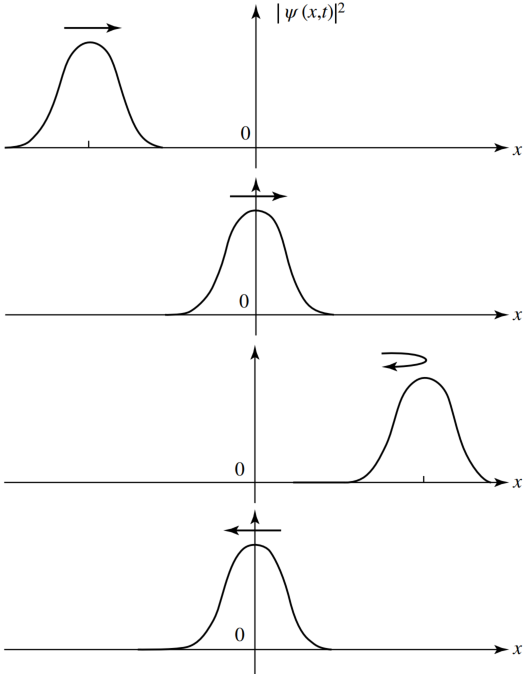
\includegraphics[width=.4\columnwidth]{PartOne/ChapterThree/gaussianalphastate.png}
    \caption{Motion of the Gaussian wave packet associated with $\ket{\alpha}$ state. Thanks to the form of $V(x)$, the wave packet oscillates without distortion.}
\end{figure}